\documentclass[a4paper,12pt]{article}
\usepackage[utf8]{inputenc}
\usepackage[brazil]{babel}
\usepackage{csquotes}
\usepackage{multirow}
\usepackage{booktabs}
\usepackage{setspace}
\usepackage{url}
\usepackage{caption}
\usepackage{biblatex}
\usepackage{acronym}
\usepackage{tocloft}
\addbibresource{referencias.bib}
\usepackage[colorlinks=true,linkcolor=black,urlcolor=blue,citecolor=blue]{hyperref}
\setstretch{1.5}
\usepackage[lmargin=3cm,tmargin=3cm,rmargin=2cm,bmargin=2cm]{geometry}
\usepackage[T1]{fontenc}
\usepackage{graphicx,xcolor,enumerate}
\usepackage{array}
\renewcommand{\cftsecleader}{\cftdotfill{\cftdotsep}}
\setlength{\cftbeforesecskip}{0.5em}
\renewcommand{\arraystretch}{1.5}
\renewcommand{\listtablename}{Lista de Tabelas}

\begin{document}
\begin{titlepage}
    \begin{center}

        %\begin{figure}[!ht]
        %\centering
        %\includegraphics[width=2cm]{c:/ufba.jpg}
        %\end{figure}

        \Huge{Instituto Federal do Piauí}\\
        \large{Departamento de Informação, Ambiente, Saúde e Produção Alimentícia}\\
        \large{Coordenação do Curso de Tecnoligia em Análise e Desenvolvimento de Sistemas}\\
        \vspace{15pt}
        \vspace{95pt}
        \textbf{\large{Desvendando a Inovação: Relatório Técnico do Desenvolvimento de Software}}\\
        \vspace{1,5cm}
        \textbf{{\LARGE{HelloPay}}}
        \vspace{3,5cm}
    \end{center}

    \begin{flushleft}
        \begin{tabbing}
            Aluno: \textbf{Vinicius Roosevelt Rodrigues Borges}\\
            Professor Orientador: Rogério da Silva\\
            %Professor co-orientador: \\
        \end{tabbing}
    \end{flushleft}
    \vspace{1cm}

    \begin{center}
        \vspace{\fill}
        Junho\\
        2023
    \end{center}
\end{titlepage}
% CAPA
\begin{titlepage}
    \begin{center}

        %\begin{figure}[!ht]
        %\centering
        %\includegraphics[width=2cm]{c:/ufba.jpg}
        %\end{figure}

        \Huge{Instituto Federal do Piauí}\\
        \large{Departamento de Informação, Ambiente, Saúde e Produção Alimentícia}\\
        \large{Coordenação do Curso de Tecnoligia em Análise e Desenvolvimento de Sistemas}\\
        \vspace{15pt}
        \vspace{45pt}
        \vspace{15pt}

        \vspace{85pt}

        \textbf{\large{Relatório Técnico de Desenvolvimento de Software}}\\
        \vspace{1,5cm}
        \textbf{\LARGE{HelloPay}}
        %	\large{Modelo\\
        %   		Validação do modelo clássico}

    \end{center}
    \vspace{1,5cm}

    \begin{flushright}

        \begin{list}{}{
                \setlength{\leftmargin}{4.5cm}
                \setlength{\rightmargin}{0cm}
                \setlength{\labelwidth}{0pt}
                \setlength{\labelsep}{\leftmargin}}

            \item Relatório Técnico de Desenvolvimento de Software apresentado para a conclusão do Curso de Tecnoligia em Analise e Desenvolvimento de Sistemas deste instituto.

                  \begin{list}{}{
                          \setlength{\leftmargin}{0cm}
                          \setlength{\rightmargin}{0cm}
                          \setlength{\labelwidth}{0pt}
                          \setlength{\labelsep}{\leftmargin}}

                      \item Aluno: Vinicius Roosevelt Rodrigues Borges
                      \item Professor Orientador: Rogério da Silva\

                  \end{list}
        \end{list}
    \end{flushright}
    \vspace{1cm}
    \begin{center}
        \vspace{\fill}
        Junho\\
        2023
    \end{center}
\end{titlepage}
\newpage



% Lista de Figuras
\listoffigures
\clearpage

% Lista de Tabelas
\listoftables
A lista de tabelas pode ser encontrada na página~ \ref{tab:casos-de-uso}.
\clearpage


    \begin{center}
        \section*{LISTA DE ABREVIATURAS E SIGLAS}
    \end{center}


    \begin{acronym}[TDMA]
        \leftskip=1in\relax\rightskip=1in\relax
        \acro{API}{Interface de Programação de Aplicativos}
        \acro{WWW}{Rede mundial de computadores}
        \acro{UML}{Linguagem de Modelagem Unificada}
        \acro{UI}{Interface de Usuário}
        \acro{MVP}{Mínimo Produto Viável}
        \acro{UX}{Experiência do Usuário}
        \acro{HTTP}{Protocolo de Transferência de Hipertexto}
    
\end{acronym}
\newpage
\tableofcontents
\newpage

%INTRODUÇÃO
\section{INTRODUÇÃO}
\subsection{CONTEXTUALIZAÇÃO}
O Brasil tem atualmente mais de um smartphone por habitante, segundo levantamento anual divulgado pela FGV. São 242 milhões de celulares inteligentes em uso no país, que tem pouco mais de 214 milhões de habitantes, de acordo com o IBGE
\cite{celulares}.Essa estatística mostra que os smartphones se tornaram uma parte essencial do cotidiano dos brasileiros, tornando-se uma ferramenta indispensável tanto para fins pessoais quanto profissionais.Essa proliferação de dispositivos móveis cria um ambiente propício para o empreendedorismo, abrindo novas oportunidades de negócios e transformando a forma como as empresas se conectam com os consumidores.
\newline O empreendedorismo no contexto dos smartphones oferece uma ampla gama de possibilidades. Com um mercado tão grande e uma demanda crescente por serviços e aplicativos móveis, os empreendedores podem explorar diversas áreas para inovar e atender às necessidades dos usuários.
Um exemplo claro é o desenvolvimento de aplicativos móveis. Com tantos smartphones em circulação, há uma demanda constante por aplicativos que ofereçam soluções úteis, entretenimento, serviços financeiros, educação, saúde e muito mais. Os empreendedores podem aproveitar essa demanda para criar e lançar aplicativos que atendam às necessidades específicas dos usuários brasileiros, seja criando novas formas de entretenimento, facilitando o acesso a serviços essenciais ou fornecendo soluções inovadoras para problemas cotidianos.
Em resumo, o Brasil está vivenciando uma realidade em que o número de smartphones ultrapassa a marca de um por habitante, oferecendo uma infinidade de oportunidades para empresas.
\newline A partir desses contexto (uso de celulares no Brasil, e novas formas de negócios através do uso de smartphones), é mais fácil para empresas criarem seus próprios aplicativo de pagamento de serviços, pois
entrega aos seus clientes uma maior integração e facilidade no momento do pagamento,dos
serviços prestados. Além de facilitar a vida dos usuários e também das empresas, fazendo
com que o foco de uma empresa seja em outras áreas que possibilitam um maior conforto
na hora de gerência/pagamento dos serviços prestados. Para contribuir com essas empresas é proposto um software mobile para dar dinamicidade para esses pagamentos, mas também um interface confortável para empresa e seu usuário

\subsection{JUSTIFICATIVA}
Na Atualidade  é muito difícil para pessoas que tão iniciando na vida do empreendedorismo ou já são micro-empresas nascerem grande e concorrerem com outras empresas, logo para se destacar no mercado é obrigatório trabalhar no diferencial de que as  concorrentes não oferecem, mantendo assim um padrão de qualidade, logo esse software impacta positivamente na qualidade de atendimento,porquê através de poucos cliques o usuário já estará fazendo o pagamento de um serviço e usufruindo sem precisar ligar para um atendente ou até mesmo o dono do negócio,desse empreendedor ou da micro empresas que estão procurando ter dinamicidade na empresa ou no pequeno negócio.
Seguindo essa ideia, esse software busca criar também soluções de pagamento para que seja ofertado a empresa um app de gerenciamento (acompanhamento das assinaturas de um cliente) de pagamento, para que assim haja facilidade na hora da comprança dos clientes e pagamento por eles.A administração de pagamentos em aplicativos mobile refere-se à capacidade de processar e facilitar transações financeiras dentro do contexto de um aplicativo móvel.Essa funcionalidade é fundamental para aplicativos que oferecem serviços de comércio eletrônico, assinaturas, serviços on-demand, entre outros.
\subsection{OBJETIVOS}
\subsubsection{Objetivo Geral}
Solução de Software para gestão de pagamento de um serviço,ao criar um software mobile, permite-se criar uma integração de recursos de gestão de pagamentos permitindo usuários realizem transações de forma conveniente e segura diretamente pelo aplicativo, o que também contribui para que o dono do software consigar agradar seus clientes, e ter maior controle sobre o seu negócio,possibilitando assim uma melhoria na área de serviços da sua empresa ou pequeno negócio.
\subsubsection{Objetivos Específicos}
\begin{itemize}
    \item Gestão de Pagamentos desacoplado (e com possiblidades de novas integrações de pagamentos) que possibilita as ações de criação, emissão e acompanhamento de compensação em diversas modalidades, tais como Cartão, PIX e Boleto.
    \item Disponibilizar um Sistema Mobile para tornar o aplicativo mais acessível para as Empresas.
    \item Oferecer uma experiência de compra ou pagamento integrada, sem a necessidade de redirecionar os usuários para sites externos ou aplicativos de terceiros.
\end{itemize}
\section*{Resumo}

\hspace{0.5cm}Neste capítulo,foi apresentado uma introdução sobre os aumentos do uso de celulares no Brasil,como justificativa para a criação de um aplicação mobile.Logo depois,foi mostrada a justificativa do trabalho em si,que se concentra na ideia dos benéficios a união  dos temas celulares e como a tecnologia pode trazer benéficios para empresas de menores porte concorrerem com as grandes no mercado,centrado na temática Gestão de Pagamentos.Por
último, foram pontuados os objetivos geral e específicos do projeto.

\hspace{0.5cm}Os próximos capítulos estão apresentados na seguinte sequência:
\begin{itemize}
    \item \textbf{Fundamentação Teórica:} Capítulo voltado para a exibição dos conceitos teóricos
          utilizados no desenvolvimento da solução proposta no trabalho;
    \item \textbf{Metodologia:} Capítulo dedicado a apresentação da metologia utilizada na criação
          do projeto da solução, através do levantamento de requisitos do software proposto,
          da listagem das ferramentas que foram e das que serão utilizadas, e apresentação do
          projeto de aplicação.
    \item \textbf{Conclusão:} Capítulo direcionado a conclusão do projeto, com a sugestão de trabalhos
          futuros, os quais se resumem a iniciar o desevolvimento prático da solução.
\end{itemize}
%FUNDAMENTAÇÃO TEORICA
\newpage

\section{FUNDAMENTAÇÃO TEÓRICA}
\subsection{TECNOLOGIA,EMPRENDEDORISMO E PAGAMENTOS}
Com o advento das redes sociais, a exemplo do Orkut, em janeiro de 2004, a internet ganhou outros contornos,começou a gerar novos empregos, novas empresas sugiram no ramo da tecnologia, o marketing digital começou a ganhar força, os bancos começaram a ter novas formas de transações. Toda essa mudança proporcionada pela internet começou com o aparecimento de sites como Kazaa e P2P, que tinham como propósito compartilhar dados, o que deu abertura para a entrada de outras comunidades online, como Twitter, Skype, Orkut e, mais recentemente, o Facebook e o Instagram. As redes sociais evoluíram tanto ao longo do tempo que hoje também são utilizadas para negócios \cite{internet}.
Um oportunidade interessante é a economia compartilhada, impulsionada por aplicativos móveis. Plataformas de compartilhamento de caronas, aluguel de imóveis e serviços diversos têm se tornado cada vez mais populares, permitindo que empreendedores criem negócios baseados na conexão entre usuários e provedores de serviços. Essa abordagem tem o potencial de transformar setores inteiros da economia, gerando oportunidades para empreendedores inovadores.
O mundo dos pagamentos é um ecossistema complexo e diversificado que envolve várias partes e tecnologias para facilitar as transações financeiras entre indivíduos, empresas e instituições.Geralmente os Pagamentos Giram em Torno de alguns atores:Participantes,Modalidades de Pagamento,Processamento do pagamento e Segurança.
\subsubsection{Participantes}
Geralmente são pessoas ou empresas que realizam pagamentos para adquirir bens ou serviços
\subsubsection{Modalidades de Pagamento}
Vária desde a dinheiro em espécie há cartões de crédito/débito e criptomoedas.
\subsubsection{Processamento do pagamento}
São comumentes conhecidos como os status(estado de uma transação).
\begin{itemize}
    \item Autorização: O processo de verificação e validação do pagamento pelo emissor do cartão ou instituição financeira envolvida.
          utilizados no desenvolvimento da solução proposta no trabalho;
    \item Liquidação: Transferência do valor do pagamento do cliente para o comerciante, geralmente por meio das instituições financeiras envolvidas.
    \item Compensação: Verificação das transações e ajuste dos saldos entre as instituições financeiras.
    \item Conciliação: Processo de reconciliação entre as transações registradas pelos comerciantes e as transações processadas pelas instituições financeiras.
\end{itemize}
\subsubsection{Segurança}
Garante que dados sensiveis não sejam expostos
\begin{itemize}
    \item Criptografia: Uso de algoritmos criptográficos
    \item Tokenização: Substituição dos dados sensíveis por um token único
    \item Autenticação: Verificação da identidade do cliente por meio de senhas, códigos de segurança, biometria, entre outros.
    \item Monitoramento: Uso de sistemas e tecnologias para identificar atividades suspeitas e prevenir fraudes.
\end{itemize}
É importante destacar que o mundo dos pagamentos está em constante evolução, impulsionado pelo avanço tecnológico e pela demanda por soluções mais rápidas, seguras e convenientes. Novas tecnologias, como blockchain, inteligência artificial e Internet das Coisas, estão sendo aplicadas para melhorar os processos de pagamento e proporcionar experiências mais eficientes aos usuários.
\newpage
\subsection{DIAGRAMA DE CLASSES}
Diagrama de classes é um tipo de diagrama \ac{UML} muito usado para demonstrar as relações de classes que serão usados para modelagem de objetos quando o código for gravado.
A forma de classe em si consiste em um retângulo
com três linhas. A linha superior contém o nome da classe,
a linha do meio, os atributos da classe e a linha inferior expressa os
métodos ou operações que a classe pode utilizar. Classes e subclasses
são agrupadas juntas para mostrar a relação estática entre cada objeto.\cite{diagramaclasse}.
Decerto existem alguns benefícios em utilizar o diagrama de classes, dentre eles, ilustrar
modelos de dados para sistemas, sejam eles simples ou complexos, e expressar visualmente as
necessidades de um sistema \cite{diagramaclasse}.
\subsection{CASOS DE USO}
Os casos de usos são um tipo de diagrama comportamental de \ac{UML} \cite{casodeusos}, usando para descrever os detalhes das funcionalidades e interação com um sistemas.
Indentifica-se várias ultilidades neses diagrama desde a documentação dos detalhes de um software, permitir melhor entendimento do fluxo feito no sistema e além de dar melhores detalhes para o desenvolvedor que vai implementar.
Existe ainda uma estrutura de especificação do caso de uso, com mais detalhes sobre
o mesmo. É possível modificar a estrutura de tópicos conforme necessário em cada situação.
Os diagramas de caso de uso consistem em 4 objetos:Ator,Caso de uso,Sistema,Pacote \cite{casodeusos}.
Embora os diagramas de caso de uso possam ser usados para vários fins, há algumas diretrizes comuns que você precisa seguir ao desenhar casos de uso.

Estes incluem padrões de nomear, direções de setas, colocação de casos de uso, uso de caixas de sistema e também uso adequado de relacionamentos \cite{casodeusos}.
\subsection{FIGMA}
Figma é um software para edição de designs gráficos, vetores e protótipos, baseado em nuvem, que permite a criação de artes individualmente ou de forma colaborativa em tempo real,
e, desde então, permite que designers e desenvolvedores se comuniquem e transfiram produtos criados através de códigos com maior agilidade e facilidade \cite{figma}, as que se destacam são:
versionamento automático, painel de camadas e objetos, biblioteca compartilhável de componen-
tes, possibilidade de compartilhar o projeto e colocá-lo em modo de apresentação, e também
permite criar fluxo de navegação entre telas.
\subsection{VISUAL STUDIO CODE}
O Visual Studio Code é um editor de código-fonte lançado em 2015 e desenvolvido pela
empresa Microsoft \cite{vscode}. A IDLE é baseada no framework Electron e está disponível para diferentes
plataformas de sistemas operacionais Windows, Linux e macOS.
É uma ferramenta que vem com suporte integrado para algumas linguagens de programa-
ção, bem como uma variada lista de extensões para outras linguagens \cite{vscode}. Além de conta com ferramentas de versionamento de código como Git
\subsection{GIT E GITHUB}
São dois software que atuam junto o Git como orquestrador e o GitHub como armazenador entre outras gestões de código. Primeiramente, o Git é um
sistema de controle de versão distribuído \cite{git}, e um recurso que o destaca dentre os outros do
mesmo tipo é seu recurso de ramificações, as quais podem ser independentes entre si, ou seja,
pode ser feita uma alteração em uma ramificação específica e não vai haver mudanças nas outras.
Já o GitHub é um local de hospedagem de código-fonte e arquivos com controle de
versão utilizando o Git \cite{github}.
\subsection{DART}
Dart é uma linguagem de programação usada para desenvolver aplicações de várias plataformas a partir do mesmo código fonte. Ela foi criada pela empresa Google em 2011 \cite{dart}.
É uma linguagem fortemente tipada que auxilia no desenvolvimento de software e evitar erros de sintaxe,
Porém, também possui desvantagens como ter pouco tempo de mercado
\subsection{FLUTTER}
Flutter é um framework de código aberto desenvolvido pela Google em 2015. É baseado
na linguagem de programação Dart, o que possibilita criação de aplicações para mobile, web e
desktop \cite{flutter}.
Uma grande vantagem do Flutter é sua alta produtividade, já que a mesma base de código
vai servir tanto para um aplicativo Android como para um iOS \cite{geekhunter}. Assim, não há necessidade de desenvolver uma aplicação para cada arquitetura Por isso,
grandes empresas utilizam o framework como o Nubank, iFood, Ebay e o próprio Google \cite{geekhunter}.
\subsection{JAVASCRIPT}
JavaScript (frequentemente abreviado como JS) é uma linguagem de programação
interpretada estruturada, de script em alto nível com tipagem dinâmica fraca e
multiparadigma (protótipos, orientado a objeto,
imperativo e funcional) \cite{javascript}.
\subsection{TYPESCRIPT}
TypeScript é uma linguagem de programação de código aberto desenvolvida pela
Microsoft. É um superconjunto sintático estrito de JavaScript e adiciona tipagem
estática opcional à linguagem. Tipos fornecem uma maneira de descrever a forma de
um objeto, fornecendo melhor documentação e permitindo que o TypeScript valide
se seu código está funcionando corretamente.
Como TypeScript é um superconjunto de JavaScript, os programas JavaScript existentes também são programas TypeScript válidos \cite{typescript}.
\subsection{NODE}
Node.js é um ambiente de execução JavaScript que permite executar aplicações desenvolvidas com a linguagem de
forma autônoma, sem depender de um navegador. Com ele, é possível criar
praticamente qualquer tipo de aplicações web, desde servidores para
sites estáticos e dinâmicos, até APIs e sistemas baseados em microserviços \cite{node}.
\subsection{API}
A sigla \ac{API} deriva da expressão inglesa Application Programming Interface que, traduzida para o português, pode ser compreendida como uma interface de programação de aplicação. Ou seja, \ac{API} é um conjunto de normas que possibilita a comunicação entre plataformas por meio de uma série de padrões e protocolos.
Por meio de APIs, desenvolvedores podem criar novos softwares e aplicativos capazes de se comunicar com outras plataformas. Por exemplo: caso um desenvolvedor queira criar um aplicativo de fotos para Android, ele poderá ter acesso à câmera do celular através da \ac{API} do sistema operacional, sem ter a necessidade de criar uma nova interface de câmera do zero \cite{api}.
\subsection{REST}
Na informática e engenharia de software, Representational State Transfer (abreviado REST), em português Transferência de Estado Representacional, é um estilo de arquitetura de software, criado em 2000 por Roy Fielding, que define um conjunto de restrições a serem usadas para a criação de um tipo especial de serviços-Web, denominados Web services RESTful, que fornecem interoperabilidade entre sistemas de computadores na Internet; RESTful permite que os sistemas solicitantes acessem e manipulem representações textuais de recursos da Web usando um conjunto uniforme e predefinido de operações sem estado (requisição e resposta independentes). Outros tipos de Web services, como Web services SOAP, expõem seus próprios conjuntos de operações arbitrários \cite{rest}.
\subsection{POSTGRES}
O PostgreSQL é um banco de dados relacional de software livre com suporte de 30 anos
de desenvolvimento, sendo um dos bancos de dados relacionais mais estabelecidos
disponíveis. A popularidade do PostgreSQL com desenvolvedores e administradores se
deve à sua flexibilidade e integridade notáveis. Por exemplo, o PostgreSQL dá
suporte a consultas relacionais e não relacionais, além de que sua natureza de
software livre significa uma comunidade dedicada de mais de 600 colaboradores
que melhora constantemente o sistema de banco de dados \cite{postgres}.

%Metodologia
\section{METODOLOGIA}
\hspace{0.5cm}A metodologia do projeto foi feita em três momentos. Primeiramente, com o levanta-
mento dos requisitos do software, que definiu os serviços que o software oferecerá. Em seguida,
é abordada quais ferramentas foram e quais serão utilizadas no desenvolvimento da aplicação.
Por fim, é apresentada a aplicação, com suas caraterísticas e fluxo de telas.
\subsection{LEVANTAMENTO DE REQUISITOS}
\hspace{0.5cm}O levantamento de requisitos para o desenvolvimento do projeto, foi feito através de dois
itens: diagrama de classes e casos de uso.
\clearpage
\subsubsection{Diagrama de classes}
\hspace{0.5cm}Nesse tópico, foi aplicado o diagrama de classes, para exibir as classes presentes no
sistema e seus respectivos atributos e métodos.

\begin{figure}[ht!]
    \centering
    \caption{Figura 1: Diagrama de Classe}
    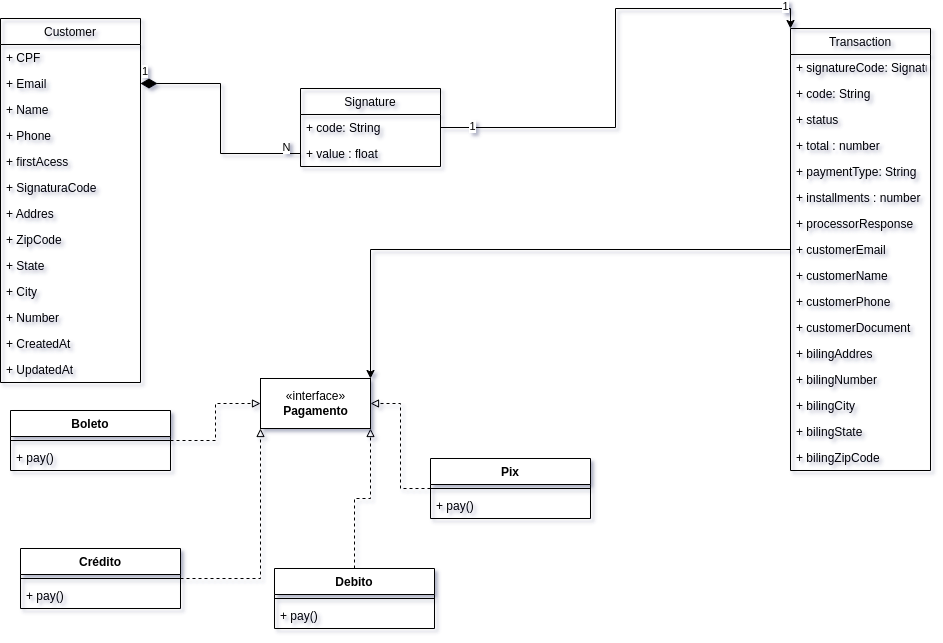
\includegraphics[width=15cm]{imagens/diagrama de Classe.png}
    \textbf{Fonte:} Elaborada pelo Autor
\end{figure}

\hspace{0.5cm}Primeiramente,o usuário pode assumir o papel de Admin ou Cliente,nunca os dois ao mesmo tempo, que define desempenham funções diferentes no sistema.
Adiante, as assinaturas faz o papel de gestor entre as transações e o cliente, logo um cliente pode ter apenas uma assinatura e assinatura pode pertencer a diferentes clientes,
Ademais, as transações recebem uma assinatura e dados de um cliente para serem realizadas e dependendo da interface de pagamento recebe essa transações seus atributos podem ser alterados
Por fim, a interface de pagamento depende do tipo de pagamento que o cliente deseja fazer, assim se adaptando a diferentes contextos de pagamentos

\newpage
\subsubsection{Casos de uso}
\hspace{0.5cm}Nesse item, foram utilizados os casos de uso, uma forma existente para especificar
as funcionalidades do software. Nas tabelas abaixo, foram abordadas sobre cada função o
ator principal, a descrição, o propósito, a pré-condição, o fluxo principal, e, se existir, o fluxo
alternativo e o fluxo exceção.
%Use Case 01
\begin{table}[ht]
    \centering
    \begin{tabular}{|p{3.5cm}|p{10cm}|p{7cm}|}
        \hline
        \textbf{UC-01}                  & \textbf{EFETUAR LOGIN}                                                           \\
        \hline

        \multirow{1}{*}{Ator principal} & Usuário                                                                          \\
        \hline
        \multirow{1}{*}{Descrição}      & Autenticação do usuário cadastrado no sistema, permitindo a realização
        de operações na área restrita do site.                                                                             \\
        \hline

        \multirow{1}{*}{Propósito}      & Acessar o sistema para ver pagamentos, sua assinatura..                          \\
        \hline

        \multirow{1}{*}{Pré-condição}   & O usuário deve estar cadastrado no sistema..                                     \\
        \hline

        \multirow{1}{*}{Fluxo principal}
                                        & Entrar pelo login;                                                               \\
                                        & O sistema solicita informações obrigatórias para a autenticação: e-mail e senha; \\
                                        & O usuário informa os dados de autenticação;                                      \\
                                        & O sistema habilita as ações relacionadas ao software.                            \\
        \cline{2-2}
        \hline

        \multirow{2}{*}{Fluxo Alternativo}
                                        & Opção voltar                                                                     \\
                                        & • O usuário seleciona a opção voltar;                                            \\
                                        & • O sistema retorna a tela anterior.                                             \\
                                        & • O usuário seleciona a opção esqueci a senha;                                   \\
                                        & • O sistema mostra uma tela para atualizar a senha;                              \\
                                        & • O usuário informa a nova senha;                                                \\
                                        & • A senha é atualizada;                                                          \\
                                        & • O sistema retorna a página de login.                                           \\
        \hline
        \multirow{2}{*}{Fluxo de Exceção}
                                        & Informações obrigatórias para a autenticação incorretas:                         \\
                                        & • O sistema informa ao usuário o erro.                                           \\
        \hline
    \end{tabular}
    \caption{Tabela de Caso de Uso de Realizar Login}
    \label{tab:casos-de-uso}
\end{table}

%UseCase 02
\begin{table}[ht]
    \centering
    \begin{tabular}{|p{3.5cm}|p{10cm}|p{7cm}|}
        \hline
        \textbf{UC-02}                     & \textbf{Realizar cadastro}                                                               \\
        \hline

        \multirow{1}{*}{Ator principal}    & Admin                                                                                    \\
        \hline
        \multirow{1}{*}{Descrição}         & Cadastro do cliente, que vai permitir o login e acesso ao software.                      \\
        \hline

        \multirow{1}{*}{Propósito}         & Acessar o sistema para ver pagamentos, sua assinatura..                                  \\
        \hline

        \multirow{1}{*}{Pré-condição}      & O Cliente deve ter email unico, que não consta na base de dados e informações válidas    \\
                                           & Admin Deve conhecer uma senha especial para fornecer ao sistema                          \\
        \hline

        \multirow{1}{*}{Fluxo principal}
                                           & • Entrar pelo login;                                                                     \\
                                           & • O sistema retorna a página inicial e possuindo a opção de cadastrar novos clientes com \\
                                           & • O Admin informa os dados de cadastro;                                                  \\
                                           & • O sistema habilita as ações relacionadas ao software para o usuário.                   \\
        \cline{2-2}
        \hline

        \multirow{1}{*}{Fluxo Alternativo} & N/A                                                                                      \\
        \hline

        \multirow{2}{*}{Fluxo de Exceção}
                                           & Campos obrigatórios                                                                      \\
                                           & • O sistema verifica que os campos obrigatórios não forma preenchi-
        dos;                                                                                                                          \\
                                           & • O sistema exibe mensagem de alerta.                                                    \\
                                           & E-mail já existente                                                                      \\
                                           & • O sistema verifica que o e-mail informado já está cadastrado no
        sistema;                                                                                                                      \\
                                           & • O sistema exibe mensagem de alerta.                                                    \\
        \hline
    \end{tabular}
    \caption{Tabela de Caso de Uso de Realizar Cadastro}
\end{table}
%UseCase 03
\begin{table}[ht]
    \centering
    \begin{tabular}{|p{3.5cm}|p{10cm}|p{7cm}|}
        \hline
        \textbf{UC-03}                     & \textbf{Realizar cadastro de uma Assinatura}                                                                     \\
        \hline

        \multirow{1}{*}{Ator principal}    & Admin                                                                                                            \\
        \hline
        \multirow{1}{*}{Descrição}         & Cadastro das assinaturas, que permite indentificar o plano do usuário                                            \\
        \hline

        \multirow{1}{*}{Propósito}         & Permitir o usuário paga sua assinatura..                                                                         \\
        \hline

        \multirow{1}{*}{Pré-condição}      & O Admin deve está logado para criar as assinaturas                                                               \\
        \hline

        \multirow{1}{*}{Fluxo principal}
                                           & • Entrar pelo login;                                                                                             \\
                                           & • A Home Possui um botão que indica a criação de assinaturas                                                     \\
                                           & • O Admin informa os dados da assinatura;                                                                        \\
                                           & • O sistema habilita as ações relacionadas ao usuário poder tem aquela assinatura.                               \\
        \cline{2-2}
        \hline

        \multirow{1}{*}{Fluxo Alternativo} & N/A                                                                                                              \\
        \hline

        \multirow{2}{*}{Fluxo de Exceção}
                                           & Caso o Admin não esteja logado ou quem quer criar a assinatura não seja admin                                    \\
                                           & • O Sistema verifica a identidade do usuário e caso ele não seja admin não deixa continuar e exibi uma mensagem; \\
                                           & • O sistema exibe mensagem de alerta.                                                                            \\
        \hline
    \end{tabular}
    \caption{Tabela de Caso de Uso de Criar uma Assinatura}
\end{table}

%UseCase 04
\begin{table}[ht]
    \centering
    \begin{tabular}{|p{3.5cm}|p{10cm}|p{7cm}|}
        \hline
        \textbf{UC-04}                     & \textbf{Apagar nos registro  uma Assinatura}                                                                                                                              \\
        \hline

        \multirow{1}{*}{Ator principal}    & Admin                                                                                                                                                                     \\
        \hline
        \multirow{1}{*}{Descrição}         & Excluir dos registros uma assinatura que não faz mais parte do contexto do sistema                                                                                        \\
        \hline

        \multirow{1}{*}{Propósito}         & Manter Limpo os Registros que não vão mais ser ultilizados..                                                                                                              \\
        \hline

        \multirow{1}{*}{Pré-condição}      & O Admin deve está logado para apagar as assinaturas                                                                                                                       \\
        \hline

        \multirow{1}{*}{Fluxo principal}
                                           & • Entrar pelo login;                                                                                                                                                      \\
                                           & • A Home Possui um botão que leva para ver todas as assinaturas e caso o haja a necessidade de excluir a assinatura é apagada do sistemas sem prejudicar outras entidades \\
        \cline{2-2}
        \hline

        \multirow{1}{*}{Fluxo Alternativo} & N/A                                                                                                                                                                       \\
        \hline

        \multirow{2}{*}{Fluxo de Exceção}
                                           & Caso o Admin não esteja logado ou Usuário qualquer deseje apagar a assinatura                                                                                             \\
                                           & • O Sistema verifica a identidade do usuário e caso ele não seja admin não deixa continuar                                                                                \\
                                           & • O sistema exibe mensagem de alerta.                                                                                                                                     \\
        \hline
    \end{tabular}
    \caption{Tabela de Caso de Uso de Apagar uma Assinatura}
\end{table}
%UseCase 05
\begin{table}[ht]
    \centering
    \begin{tabular}{|p{3.5cm}|p{10cm}|p{7cm}|}
        \hline
        \textbf{UC-05}                     & \textbf{Alterar dos registros uma Assinatura}                                              \\
        \hline

        \multirow{1}{*}{Ator principal}    & Admin                                                                                      \\
        \hline
        \multirow{1}{*}{Descrição}         & Alterar dos registros uma assinatura que atualizando o seu contexto no sistema             \\
        \hline

        \multirow{1}{*}{Propósito}         & Manter as assinaturas de acordo com o contexto do software..                               \\
        \hline

        \multirow{1}{*}{Pré-condição}      & O Admin deve está logado para alterar as assinaturas                                       \\
        \hline

        \multirow{1}{*}{Fluxo principal}
                                           & • Entrar pelo login;                                                                       \\
                                           & • A Home Possui um botão que leva para ver todas as assinaturas                            \\
                                           & • E nessa listagem possui o botão de alterar assinatura                                    \\
                                           & • O Admin informa os campos a serem alterados                                              \\
                                           & • Por fim o Admin salva as alterações                                                      \\
        \cline{2-2}
        \hline

        \multirow{1}{*}{Fluxo Alternativo} & N/A                                                                                        \\
        \hline

        \multirow{2}{*}{Fluxo de Exceção}
                                           & Caso o Admin não esteja logado ou Usuário qualquer deseje alterar alguma  assinatura       \\
                                           & • O Sistema verifica a identidade do usuário e caso ele não seja admin não deixa continuar \\
                                           & • O sistema exibe mensagem de alerta.                                                      \\
        \hline
    \end{tabular}
    \caption{Tabela de Caso de Uso de Alterar uma Assinatura}
\end{table}
%UseCase 06
\begin{table}[ht]
    \centering
    \begin{tabular}{|p{3.5cm}|p{10cm}|p{7cm}|}
        \hline
        \textbf{UC-06}                     & \textbf{ Listar dos registros todas as Assinaturas}                                        \\
        \hline

        \multirow{1}{*}{Ator principal}    & Admin                                                                                      \\
        \hline
        \multirow{1}{*}{Descrição}         & Visualiza dos registros todas as Assinaturas do Sistema                                    \\
        \hline

        \multirow{1}{*}{Propósito}         & Visualizar todas as Assinaturas do Software                                                \\
        \hline

        \multirow{1}{*}{Pré-condição}      & O Admin deve está logado para visualizar todas as assinaturas                              \\
        \hline

        \multirow{1}{*}{Fluxo principal}
                                           & • Entrar pelo login;                                                                       \\
                                           & • A Home Possui um botão que leva para ver todas as assinaturas                            \\
                                           & • E nessa nova tela é possível ver todas as assinaturas                                    \\
        \cline{2-2}
        \hline

        \multirow{1}{*}{Fluxo Alternativo} & N/A                                                                                        \\
        \hline

        \multirow{2}{*}{Fluxo de Exceção}
                                           & Caso o Admin não esteja logado ou Usuário qualquer deseje visualizar todas as  assinaturas \\
                                           & • O Sistema verifica a identidade do usuário e caso ele não seja admin não deixa continuar \\
                                           & • O sistema exibe mensagem de alerta.                                                      \\
        \hline
    \end{tabular}
    \caption{Tabela de Caso de Uso de Visualizar todas  as Assinaturas}
\end{table}
%UseCase 07
\begin{table}[ht]
    \centering
    \begin{tabular}{|p{3.5cm}|p{10cm}|p{7cm}|}
        \hline
        \textbf{UC-07}                     & \textbf{Criar uma Transação}                                                                \\
        \hline

        \multirow{1}{*}{Ator principal}    & Usuário                                                                                     \\
        \hline
        \multirow{1}{*}{Descrição}         & O Usuário está preparando o caminho para pagar sua assinatura                               \\
        \hline

        \multirow{1}{*}{Propósito}         & Realizar o pagamento da assinatura                                                          \\
        \hline

        \multirow{1}{*}{Pré-condição}      & O Usuário deve está logado, e possuí uma assinatura                                         \\
        \hline

        \multirow{1}{*}{Fluxo principal}
                                           & • Entrar pelo login;                                                                        \\
                                           & • A Home Possui que levar o usuário a visualizar sua assinatura                             \\
                                           & • Caso ele queria ele pode efetuar o pagamento de sua assinatura                            \\
                                           & • Criando uma Transação no Sistema                                                          \\
                                           & • Que fica ouvindo as modifiações caso haja um  pagamento daquela transação                 \\
        \hline

        \multirow{1}{*}{Fluxo Alternativo} & Caso o Usuário não deseje continuar                                                         \\
                                           & • É criado a transação,porém com status de cancelada pelo usuário                           \\
        \hline

        \multirow{1}{*}{Fluxo de Exceção}
                                           & Caso o email informado não for o mesmo que do usuário                                       \\
                                           & • A transação é cancelada                                                                   \\
                                           & • O Sistema verifica a identidade do usuário e do email passado para criacão da transaction \\
                                           & • O sistema exibe mensagem de alerta.                                                       \\
        \hline
    \end{tabular}
    \caption{Tabela de Caso de Uso de Criar uma transação}
\end{table}

%UseCase 08
\begin{table}[ht]
    \centering
    \begin{tabular}{|p{3.5cm}|p{10cm}|p{7cm}|}
        \hline
        \textbf{UC-08}                     & \textbf{ Altera o Status de uma Transanção de Pendente para Pago}                                                           \\
        \hline

        \multirow{1}{*}{Ator principal}    & Sistema                                                                                                                     \\
        \hline
        \multirow{1}{*}{Descrição}         & Quando o Sistema é notificado é alterado o status da transação do Usuário                                                   \\
        \hline

        \multirow{1}{*}{Propósito}         & Atualizar o Status da Transação para Pago                                                                                   \\
        \hline

        \multirow{1}{*}{Pré-condição}      & O usuário deve ter feito iniciado o pagamento da Transação e ter seguido as etapas de colocar seus dados para o pagamento   \\
        \hline

        \multirow{1}{*}{Fluxo principal}   & • O Sistema é notificado que o usuário quer fazer o pagamento e muda o status de Iiniciado para Pendente                    \\
                                           & • O Cliente Paga a Transação                                                                                                \\
                                           & • A Gateway de Pagamento notificar o sistema                                                                                \\
                                           & • E Alterar status de Pendente para Pago                                                                                    \\
        \hline

        \multirow{1}{*}{Fluxo Alternativo} & N/A                                                                                                                         \\
        \hline

        \multirow{1}{*}{Fluxo de Exceção}
                                           & Caso o usuário não insira dados validos para o pagemnto ou não foi houve algo problema de saldo                             \\
                                           & • A transação volta para o status  de Pendente                                                                              \\
                                           & • O Sistema exibe uma mensagem para o usuário de alerta avisando o ocorrido                                                 \\
                                           & Caso haja algum problema com o Sistema ou Gateway                                                                           \\
                                           & • O Sistema verifica o Erro                                                                                                 \\
                                           & • Caso seja problema na gateway o status fica pendente até o sistema ser notificado que houve sucesso ou falha na transação \\
                                           & • Caso seja sucesso para aprovado                                                                                           \\
                                           & • Caso seja falha para erro                                                                                                 \\
                                           & • O Sistema mostra uma mensagem de erro ou sucesso                                                                          \\

        \hline
    \end{tabular}
    \caption{Tabela de Caso de Uso de Alterar Status de Uma Transação}
\end{table}

\clearpage
%Ferramentas
\subsection{FERRAMENTAS}
Essa seção compartilha,todas as \textbf{coisas} que contribui e contribuirão para criação do software, que váriam desde a linguagem de progamação,criação de \ac{UI},frameworks, e criação de diagramas.

\subsubsection{Ferramentas utilizadas}
\begin{itemize}
    \item \textbf{Node}: Adotado como motor do JavaScript, que permite a execução do Javascript fora de um navegador web,possibilitando o desenvolvimento de aplicativos do lado do servidor.
    \item \textbf{TypeScript}: Aplicado devido a ser uma linguagem de progamação tipada, o que dar vantagens para o compilador enterpretar melhor variáveis,métodos e classes,dando melhor produtividade.
    \item \textbf{JavaScript}: Após o projeto ser publicado o TypeScript e transpilado em JavaScript para poder rodar no motor do Node.
    \item \textbf{Draw.io}: Empregado para criação de diagrmas online como os da \ac{UML}, sendo um editor de diagrams de código aberto que permite criar uma gama de outros diagramas
    \item \textbf{Postgres}: Postgres, é um sistema de gerenciamento de banco de dados relacional de código aberto. Ele é conhecido por sua confiabilidade, escalabilidade e recursos avançados, tornando-se uma escolha popular para muitas aplicações e projetos.
\end{itemize}
\subsubsection{Ferramentas a Serem utilizadas}
\begin{itemize}
    \item \textbf{Dart}: O Dart é uma linguagem moderna e eficiente, com suporte a recursos como tipagem estática, gerenciamento de memória eficiente e compilação just-in-time (JIT) para um desenvolvimento e execução rápidos.
    \item \textbf{Flutter}: Flutter é um framework de código aberto desenvolvido pelo Google, usado para criar aplicativos nativos de alta qualidade para dispositivos móveis, web e desktop. Ele permite que os desenvolvedores escrevam o código uma vez e o executem em diferentes plataformas, utilizando uma única base de código.
    \item \textbf{Figma}: O Figma é uma plataforma de design de interface do usuário \ac{UI} e experiência do usuário \ac{UX} baseada na nuvem.
    \item \textbf{Draw.io}: Empregado para criação de diagrmas online como os da \ac{UML}, sendo um editor de diagrams de código aberto que permite criar uma gama de outros diagramas
    \item \textbf{Postgres}: Postgres, é um sistema de gerenciamento de banco de dados relacional de código aberto. Ele é conhecido por sua confiabilidade, escalabilidade e recursos avançados, tornando-se uma escolha popular para muitas aplicações e projetos.
\end{itemize}
\section{HelloPay}
\hspace{0.5cm}O HelloPay tem a proposta de ser mobile e somente para android inicialmente.Do mesmo modo, o sofware será baseado em interfaces famosas como nubank,ifood,uber,entre outros aplicativos, devido a ter uma interface boa e rápida para o usuário.A ideia é juntar o crescente uso dos celulares com empreendedorismo e pagamentos que possibilite a empresas menores competirem com as grandes.
\subsection{Resultados}
\hspace{0.5cm}Essa seção é reservada para demonstrar os resultados dos casos de usos unidos e alguns detalhes singelos da aplicação,como arquitetura do sistema e como ele é divido e a função de cada parte dele.
\newline A aplicação HelloPay tem como objetivo ser um app voltado para  gestão de pagamentos, esse app é altamente flexível, permitindo a integração de novos métodos de pagamento de forma independente. Ele oferece funcionalidades abrangentes para a criação, emissão e acompanhamento de transações em diversas modalidades, incluindo Cartão, PIX e Boleto. O sistema é dividido em três partes principais, que garantem um fluxo eficiente e seguro de pagamentos.
\newpage
\begin{figure}[ht!]
    \centering
    \caption{Estrutura do Software}
    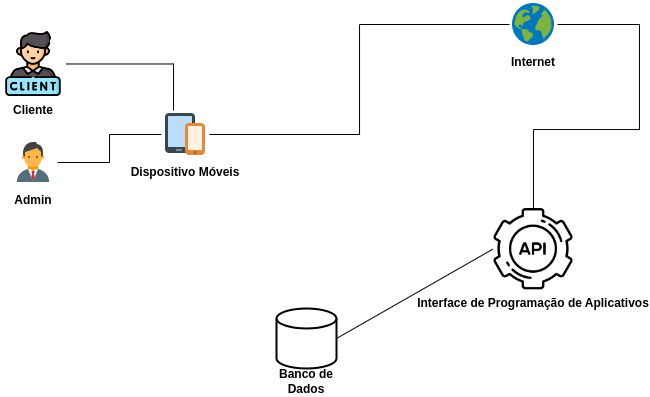
\includegraphics[width=15cm]{imagens/Estrutura do software.drawio.png}
    \textbf{Fonte:} Elaborada pelo Autor
\end{figure}


\begin{itemize}
    \item \textbf{API}: As APIs são um conjunto de padrões que fazem parte de uma interface \cite{api}.A Api do HelloPay também contém conjunto de regras e protocolos que permite troca de informações entre um sistema(app de celular) para mitigar a problematica citada no Capítulo 1.Essa \ac{API} também conta com a ultilização do protocolo \ac{HTTP}, que é um protocolo muito famoso que especifica como será a comunicação entre um navegador e um servidor web,sendo um dos principais da \ac{WWW}  \cite{http}.
    \item \textbf{Aplicação móvel}: Será a parte mais ultilizada do sistema,além de conter a interface do usuário \ac{UI} além de ser o principal ponto de ligação entre o usuário e os dados providos pela \ac{API}. Será ultilizado o framework Flutter, devido ao seu desenvolvimento ser compartilhado em diferente plataformas a partir do mesmo código fonte e criação de interfaces bem concisas.
    \item \textbf{Banco de Dados}: Um sistema organizado para armazenar, gerenciar e recuperar informações de maneira estruturada. Ele é projetado para armazenar grandes quantidades de dados de forma eficiente e permitir o acesso rápido e seguro a esses dados quando necessário.
\end{itemize}
\subsection{Cronograma}
\hspace{0.5cm}Inicialmente foi criado totalmente a criação e manipulação de assinaturas,usários e transações, que já colaboram para administração de usuário e de suas transações pelo administrador além do controle dos serviços oferecidos pela empresa.As Próximas etapas para o projeto, é a produção do aplicativo mobile e conexão com gatewaty de pagamento,que possiblita fazer as transações com segurança e diferentes métodos de pagamentos, o que possiblita atingir o objetivo de pagamento desacoplado, ou seja um \ac{MVP} para já poder ser valida pelos usuários.
\newline Todo o código produzido é versionado no GitHub e cada parte do processo de contrução do software será documentada.É planejado a entrega de um aplicativo para celulares Android totalmente integrado com \ac{API} do HelloPay, além da criação de teste para garantir que as funcionalidades oferecidas pelo HelloPay são funcioanis e possui uma maior segerunça graças aos testes.

% Conclusão
\newpage
\section{CONCLUSÃO E TRABALHOS FUTUROS}
\hspace{0.5cm}Esse trabalho apresentou o projeto do aplicativo HelloPay,um app de gestão e pagamento com
foco em serviços disponibilizados por uma empresa. Para poder justificar esse trabalho,
foi feito uma pesquisa sobre o uso de celulares,a tecnologia como auxilidora do homem.
\newline Dessa forma foi proposto uma aplicação que une as duas temáticas com administração de pagamentos, um sistema de gerenciamento de pagamentos desvinculado que possibilita as etapas de criação, emissão e acompanhamento de compensação em diversas modalidades.
Primeiramente foi levantado objetivos gerais e especificos da aplicação,contribui para o gerenciamento das transações dos clientes e pagamento de serviços.
Em seguida foi realizado o levantamento de requisitos, para melhor compreensão do software.Por conseguinte foi exposto as ferramentas a serem ultilizados,desde linguagens de progamação a
frameworks e banco de dados, que foram e serão utilizadas no futuro da aplicação.
\newpage

\printbibliography
\end{document}
